\documentclass[journal]{IEEEtran}

% *** CITATION PACKAGES ***
\usepackage{cite}

% *** GRAPHICS RELATED PACKAGES ***
\usepackage{multirow,makecell}
\usepackage{booktabs, pifont}
\newcolumntype{C}[1]{>{\centering\arraybackslash}m{#1}}
\newcolumntype{L}[1]{m{#1}}
\ifCLASSINFOpdf
  \usepackage[pdftex]{graphicx}
\else
\fi

% *** MATH PACKAGES ***
\usepackage{amsmath}
\usepackage{amssymb}

% *** ALGORITHM PACKAGES ***
\usepackage{algorithm}
\usepackage{algpseudocode}

% *** ALIGNMENT PACKAGES ***
\usepackage{array}

% *** SUBFIGURE PACKAGES ***
\usepackage{subfigure}

% *** URL PACKAGES ***
\usepackage{url}
\usepackage{orcidlink}

% *** TIKZ PACKAGES ***
\usepackage{tikz}
\usetikzlibrary{positioning,shapes,arrows.meta}

% ========================================================
%  ST-MBAN: Spatio-Temporal Multi-Branch Attention Network
%  for RSU Dwell Time Prediction in CCVN
% ========================================================

\begin{document}

\title{Deterministic RSU Dwell Time Prediction via Multi-Branch Attention Network in Content-Centric Vehicular Networks}

\newcommand{\orcidauthorA}{0000-0003-3971-0715} % Youngju Nam
\newcommand{\orcidauthorC}{0000-0002-0422-0647} % Euisin Lee
\newcommand{\orcidauthorB}{0000-0001-8209-5944} % Jeong-Hun Kim

\author{Youngju Nam, Euisin Lee, and Jeong-Hun Kim

\thanks{Manuscript received April 00, 2026; revised August 00, 2026.
This work was supported by a National Research Foundation of Korea (NRF) grant funded by the Korean government (Ministry of Science and ICT (MSIT)) (No. 2022R1A2C1010121). \textit{(Corresponding author: Jeong-Hun Kim.)}}
\thanks{Youngju Nam is with the School of Software, Kunsan National University, Gunsan, Republic of Korea (e-mail: imnyj@kunsan.ac.kr).}
\thanks{Euisin Lee is with the School of Information and Communication Engineering, Chungbuk National University, Cheongju, Republic of Korea (e-mail: eslee@chungbuk.ac.kr).}
\thanks{Jeong-Hun Kim is with the Department of Computer Science and Information Engineering, Kunsan National University, Gunsan, Republic of Korea (e-mail: kimjh@kunsan.ac.kr).}
\thanks{Digital Object Identifier 10.0000/TWC.2026.0000000}}

\markboth{IEEE TRANSACTIONS ON WIRELESS COMMUNICATIONS,~Vol.~00, No.~0, 2026}%
{Youngju Nam \MakeLowercase{\textit{et al.}}: Deterministic RSU Dwell Time Prediction via Multi-Branch Attention Network in CCVNs}

\IEEEpubid{0000--0000/00\$00.00~\copyright~2026 IEEE}

\maketitle

% ============================================================
\begin{abstract}
In Content-Centric Internet of Vehicles (CIoV) networks, proactive RSU caching requires accurate prediction of vehicle dwell time at the moment a content request is issued.
The predecessor model ST-CVAE employed a Conditional Variational Autoencoder (CVAE); however, posterior collapse causes the latent variable to degenerate at training time, reducing inference to a deterministic mapping without distributional benefit.
This paper proposes \textbf{ST-MBAN} (Spatio-Temporal Multi-Branch Attention Network), a fully deterministic regression model that decomposes input features into three branches: Kinematic (K), Traffic Control (T), and Social/Contextual (S), each encoded independently to prevent gradient conflict.
Cyclical encoding resolves signal-phase discontinuities, a Squeeze-and-Excitation block provides RSU-local feature-wise attention, and a three-token multi-head self-attention layer fuses the branch representations.
Twelve SUMO-derived microscopic variables augment the feature set with fine-grained local traffic dynamics.
Experiments on SUMO-simulated CIoV environments show that ST-MBAN achieves lower MAE and RMSE than ST-CVAE and baseline ML/DL models, with ablation studies quantifying each component's marginal contribution.
\end{abstract}

\begin{IEEEkeywords}
Content-Centric Vehicular Networks, RSU Dwell Time Prediction, Multi-Branch Attention, Deterministic Regression, Event-Driven Inference, Federated Edge Learning.
\end{IEEEkeywords}

\IEEEpeerreviewmaketitle


% ============================================================
\section{Introduction} \label{sec:introduction}
% ============================================================

\IEEEPARstart{T}{he} proliferation of connected vehicles is transforming road-side infrastructure into active edge caching nodes in Content-Centric Internet of Vehicles (CIoV) networks, also referred to as Content-Centric Vehicular Networks (CCVNs) \cite{Mao2017, Ji2020IoV}.
Road-Side Units (RSUs) deliver requested content to vehicles via Vehicle-to-Infrastructure (V2I) links within a communication window spanning seconds to tens of seconds; content not locally available at the RSU at the moment of a request cannot be fully served before the vehicle exits coverage.
Proactive caching \cite{Bui2017}, placing content at the RSU before demand materializes, is essential to service continuity, and its effectiveness is gated on a single quantity: how long a specific vehicle will remain within the RSU coverage zone.
Without an accurate dwell-time estimate at the moment a content request is issued, the precaching scheduler cannot determine whether sufficient time exists to complete a transfer, nor can it prioritize among competing content requests.

Existing approaches leave three structural gaps against this requirement.
First, vehicular mobility prediction methods \cite{Altche2017, Deo2018, Yu2018STGCN, Guo2019ASTGCN} require continuous time-series inputs assembled from periodic, globally collected sensor data, and are not designed for the event-driven, single-snapshot inference setting at the RSU without incurring buffering delays incompatible with precaching latency.
Second, proactive caching research in vehicular edge networks \cite{Wang2020IoT, Wang2023Async, WangGrace2023, Jiang2024, Wang2025Informer, Khelifi2018, He2020DRL} optimizes content placement via popularity modeling or reinforcement learning, but does not produce the scalar dwell-time estimate needed to schedule individual transfers.
Third, the closest prior work on direct dwell-time prediction targets Vehicular Micro Cloud (VMC) membership \cite{VMCdwell2023} and signal-based task offloading \cite{TaskMig2023}, neither of which addresses RSU content caching, event-triggered snapshot inference, or domain-decomposed feature encoding for intersection environments.

To address these gaps, this paper proposes \textbf{ST-MBAN} (Spatio-Temporal Multi-Branch Attention Network), a deterministic dwell-time predictor designed for event-driven, RSU-local inference in CIoV environments.
When a vehicle issues a content request to its current RSU, a single snapshot of the vehicle state is captured and processed immediately, eliminating any buffering requirement.
Each RSU trains its own model instance independently from local observations, encoding inputs through three semantically separated branches: Kinematic (K), Traffic Control (T), and Social/Contextual (S), and fusing branch representations through a multi-head self-attention mechanism.

\IEEEpubidadjcol
The predecessor model ST-CVAE \cite{STCVAE} employed a Conditional Variational Autoencoder (CVAE) to model stochastic dwell-time distributions.
Empirical analysis reveals that the conditional distribution of RSU dwell time is effectively unimodal given a sufficiently informative feature vector: posterior collapse \cite{posteriorCollapse} drives the CVAE latent variable toward the prior mean during training, causing the decoder to revert to a deterministic mapping at inference without any distributional benefit.
Replacing the variational formulation with explicit deterministic regression eliminates KL annealing overhead and latent sampling latency while improving point-estimate accuracy.

The main contributions of this paper are summarized as follows:

\begin{itemize}
    \item \textbf{Deterministic prediction for dwell-time estimation.}
    We replace the CVAE formulation of ST-CVAE with a fully deterministic regression architecture.
    We provide both theoretical justification via posterior collapse analysis and empirical evidence from the ST-CVAE $\approx$ MLP equivalence.

    \item \textbf{Three-branch input decomposition.}
    We partition the input feature space into three semantically distinct branches: Kinematic (K), Traffic Control (T), and Social/Contextual (S).
    Each branch is encoded by a dedicated encoder block, preventing gradient conflict across heterogeneous variable groups.

    \item \textbf{Multi-head feature attention fusion.}
    We introduce a three-token multi-head attention mechanism over branch-level representations $[Z_k, Z_t, Z_s]$, allowing the model to weight branch contributions according to current traffic context.

    \item \textbf{SUMO-derived microscopic input variables.}
    We augment the input feature set with twelve variables obtained from the SUMO microscopic traffic simulator \cite{SUMO}, providing fine-grained local traffic dynamics unavailable from GPS-level mobility traces alone.
\end{itemize}

The remainder of this paper is organized as follows.
Section~\ref{sec:related} reviews related work on vehicular caching, mobility prediction, and dwell-time estimation.
Section~\ref{sec:system} formalizes the system model, defines the prediction task, and enumerates the input feature space.
Section~\ref{sec:architecture} describes the ST-MBAN architecture in detail.
Section~\ref{sec:experiments} presents the simulation setup, dataset collection procedure, and experimental results.
Section~\ref{sec:conclusion} concludes the paper.


% ============================================================
\section{Related Work} \label{sec:related}
% ============================================================

% ---- Category 1: Vehicular Proactive Caching ----
Research on proactive content caching in vehicular edge networks has concentrated on two primary directions: popularity-based content selection and mobility-aware cache placement \cite{Bui2017, Wang2020IoT, WangGrace2023, Chen2020Coop, Yao2021Coop}.
Early mobility-aware approaches predicted vehicle locations using trajectory models and mapped these predictions to cache placement policies at RSUs \cite{Khelifi2018, Nam2021Adaptive, Nam2023Multiple}.
More recent work integrates federated learning and deep reinforcement learning (DRL) to construct distributed caching policies while protecting vehicle privacy \cite{Wang2023Async, Jiang2024, Yu2023Mobility}.
A spatial-temporal Informer-based scheme \cite{Wang2025Informer} further captures long-range trajectory dependencies to improve cache hit ratio.
Despite these advances, none of these approaches predicts RSU dwell time as an explicit, scalar regression target; caching decisions are made indirectly through location prediction or population-level demand modeling, without knowledge of how long a specific vehicle will remain in coverage.

% ---- Category 2: Vehicular Mobility Prediction ----
Vehicular mobility prediction research encompasses trajectory forecasting and traffic flow estimation \cite{Altche2017, Deo2018, Yu2018STGCN, Guo2019ASTGCN}.
LSTM-based models \cite{Altche2017} and convolutional social pooling \cite{Deo2018} predict vehicle trajectories from continuous position sequences, while spatio-temporal graph networks \cite{Yu2018STGCN, Guo2019ASTGCN} forecast aggregate traffic flow over road graphs.
Transformer-based models \cite{Transformer2024} extend these to long-horizon trajectory prediction.
All of these methods require either continuous time-series inputs or globally aggregated sensor data, making them inapplicable to the event-driven, single-snapshot inference setting of CCVN precaching.

% ---- Category 3: Combined Caching + Dwell Time Estimation ----
A subset of work attempts to bridge mobility prediction and caching.
Digital twin frameworks \cite{DT2026} use real-time vehicle monitoring to estimate dwell times and select vehicles for cooperative caching tasks; however, this approach depends on a centralized digital twin layer and continuous monitoring rather than event-driven snapshot inference.
Traffic light-based dwell time estimation \cite{TaskMig2023} uses signal phase timing to bound vehicle sojourn for task offloading, but this is a rule-based estimation rather than a learned regression, is limited to a single variable group, specifically signal timing, and targets compute offloading rather than content caching.

% ---- Category 4: Direct Dwell Time Prediction ----
The most closely related prior work targets dwell time prediction in Vehicular Micro Cloud (VMC) environments \cite{VMCdwell2023}, where a random forest model estimates how long a vehicle will remain within a V2V cloud for task migration purposes.
While this represents the same prediction objective, critical distinctions remain: VMC dwell time is measured over a vehicle cluster rather than a fixed RSU, the model is not event-triggered by content requests, the feature set does not decompose kinematic, traffic-control, and social variables into separate encoders, and the output is not directly integrated into a content precaching scheduler.

% ---- Summary / Positioning Table ----
Table~\ref{tab:comparison} summarizes the structural comparison across representative papers under six design criteria.
\textbf{D1} (Dwell Time Prediction): the approach directly regresses RSU sojourn duration as the primary output.
\textbf{D2} (Event-Driven Snapshot): inference is triggered by a single content-request event without requiring a continuous time-series input.
\textbf{D3} (RSU-Local Learning): each RSU trains its own model from locally collected observations without a central server.
\textbf{D4} (Domain-Branch Encoding): the input feature space is partitioned into domain-specific branches, each processed by a dedicated encoder.
\textbf{D5} (Deterministic Regression): the model produces deterministic point estimates rather than stochastic samples or distributions.
\textbf{D6} (Caching Integration): the output is directly consumed by a content precaching scheduler to determine transfer feasibility.
ST-MBAN is the only approach in the surveyed literature that simultaneously satisfies all six criteria.

\begin{table*}[!t]
\centering
\caption{Structural Comparison of Representative Papers Against ST-MBAN Design Criteria}
\label{tab:comparison}
\begin{tabular}{|C{1.5cm}|C{1.3cm}|C{1.3cm}|C{1.3cm}|C{1.4cm}|C{1.3cm}|C{1.3cm}|L{5.2cm}|}
\hline
\textbf{Paper} &
\textbf{D1} &
\textbf{D2} &
\textbf{D3} &
\textbf{D4} &
\textbf{D5} &
\textbf{D6} &
\textbf{Detail} \\
\hline\hline
\cite{Wang2020IoT} & \ding{55} & \ding{55} & \ding{55} & \ding{55} & \ding{55} & Indirect &
{\small Proposes cooperative DRL for vehicular edge content caching. Maximizes cache hit ratio through joint vehicle selection and content placement. Dwell time is not estimated explicitly.} \\
\hline
\cite{Wang2023Async} & \ding{55} & \ding{55} & \ding{55} & \ding{55} & \ding{55} & Indirect &
{\small Combines asynchronous federated learning with DRL for mobility-aware cooperative cache placement. Addresses communication overhead and privacy in distributed networks. No dwell-time regression is performed.} \\
\hline
\cite{Jiang2024} & \ding{55} & \ding{55} & \ding{55} & \ding{55} & \ding{55} & Indirect &
{\small Applies asynchronous federated reinforcement learning for dynamic cache management in IoV. Handles heterogeneous vehicle speeds and content popularities. Dwell time is not modeled as a prediction target.} \\
\hline
\cite{Wang2025Informer} & \ding{55} & \ding{55} & \ding{55} & \ding{55} & Partial & Indirect &
{\small Uses a spatial-temporal Informer to capture long-range trajectory dependencies for cache-hit improvement. Mobility is inferred from periodic vehicle trajectory sequences. No scalar sojourn estimate is produced.} \\
\hline
\cite{Altche2017} & \ding{55} & \ding{55} & \ding{55} & \ding{55} & \ding{51} & \ding{55} &
{\small Predicts highway vehicle trajectories using an LSTM trained on continuous position sequences. Produces deterministic forecasts per time step. Not designed for event-triggered inference without trajectory history.} \\
\hline
\cite{Deo2018} & \ding{55} & \ding{55} & \ding{55} & \ding{55} & \ding{55} & \ding{55} &
{\small Employs convolutional social pooling to model multi-vehicle interactions for trajectory prediction. Captures lateral maneuver intent from position history. Requires a continuous sequence of past positions.} \\
\hline
\cite{Yu2018STGCN} & \ding{55} & \ding{55} & \ding{55} & \ding{55} & Partial & \ding{55} &
{\small Introduces spatio-temporal graph convolution for aggregate traffic flow forecasting over road networks. Models temporal dynamics and spatial topology jointly. Predicts flow counts rather than individual vehicle sojourn.} \\
\hline
\cite{Guo2019ASTGCN} & \ding{55} & \ding{55} & \ding{55} & \ding{55} & Partial & \ding{55} &
{\small Extends STGCN with spatial and temporal attention for adaptive traffic forecasting. Captures time-varying inter-segment correlations. Requires globally aggregated periodic sensor data.} \\
\hline
\cite{Khelifi2018} & \ding{55} & \ding{55} & \ding{55} & \ding{55} & \ding{55} & Indirect &
{\small Predicts vehicle locations using LSTM and maps predictions to proactive RSU cache placement. Targets cache-hit maximization under mobility uncertainty. Does not estimate RSU dwell time explicitly.} \\
\hline
\cite{Nam2021Adaptive} & \ding{55} & \ding{55} & Partial & \ding{55} & Partial & Indirect &
{\small Derives the optimal V2I content transfer window from predicted vehicle speed and RSU coverage geometry. RSU-local computation with analytical formula. Does not use learned dwell-time regression.} \\
\hline
\cite{Yao2021Coop} & \ding{55} & \ding{55} & \ding{55} & \ding{55} & \ding{55} & Indirect &
{\small Cooperative caching in Vehicular Content Centric Networks using social attributes and mobility. Combines social trust and trajectory prediction for cooperative content distribution. No explicit sojourn estimation.} \\
\hline
\cite{Yu2023Mobility} & \ding{55} & \ding{55} & \ding{55} & \ding{55} & Partial & Indirect &
{\small Mobility-aware proactive edge caching for large files in IoV. Uses vehicle trajectory prediction to schedule transfers before coverage is lost. Predicts vehicle positions rather than dwell duration.} \\
\hline
\cite{DT2026} & Indirect & \ding{55} & \ding{55} & \ding{55} & \ding{55} & Indirect &
{\small Constructs a digital twin layer for real-time vehicle monitoring to support cooperative caching. Indirectly infers whether a vehicle will remain for task completion. Requires centralized continuous monitoring infrastructure.} \\
\hline
\cite{VMCdwell2023} & Partial & \ding{55} & \ding{55} & \ding{55} & Partial & \ding{55} &
{\small Estimates dwell time within V2V Vehicular Micro Clouds for task migration using a random forest. Targets cluster membership duration rather than fixed-RSU sojourn. Not designed for event-triggered RSU-local inference.} \\
\hline
\cite{TaskMig2023} & Estimated & \ding{55} & \ding{55} & \ding{55} & Rule-based & \ding{55} &
{\small Estimates vehicle service window from traffic light phase data for deadline-aware task offloading. Applies a rule-based bound from signal cycle timing. Targets compute offloading rather than content caching.} \\
\hline
\textbf{ST-MBAN} & \ding{51} & \ding{51} & \ding{51} & \ding{51} & \ding{51} & \ding{51} &
{\small Proposed deterministic multi-branch attention network for event-driven RSU dwell-time prediction. Decomposes inputs into K/T/S branches with CTE and SE-block, fused via three-token MHA. Directly integrates with the content precaching scheduler.} \\
\hline
\end{tabular}
\end{table*}


% ============================================================
\section{System Model} \label{sec:system}
% ============================================================

We consider a Content-Centric Vehicular Network (CCVN) in which a set of Road-Side Units (RSUs) $\mathcal{R} = \{r_1, r_2, \ldots, r_M\}$ are deployed at fixed intervals along a road segment.
Each RSU $r_i$ maintains a circular communication coverage of radius $\rho$, enabling V2I communication with any vehicle within its range.
Vehicles traverse the road following a unidirectional mobility model, passing through successive RSU coverage zones in sequence.
At any given time instant $t$, a vehicle $v$ is associated with at most one RSU, referred to as the \emph{current RSU} $r_\text{cur}$, while the immediately subsequent RSU in the vehicle's trajectory is denoted the \emph{next RSU} $r_\text{nxt}$.

Given the vehicle's state observed at time $t_0$, the prediction task is defined as estimating two scalar dwell times: the \emph{current RSU dwell time} $\tau_\text{cur} = t_\text{cur\_out} - t_0$, representing the remaining time until the vehicle exits the coverage of $r_\text{cur}$, and the \emph{next RSU dwell time} $\tau_\text{nxt} = t_\text{nxt\_out} - t_\text{nxt\_in}$, representing the full sojourn duration within $r_\text{nxt}$.
The prediction target is thus the vector $\mathbf{y} = [\tau_\text{cur},\, \tau_\text{nxt}]^\top \in \mathbb{R}^2$.

Prediction is triggered exclusively by content request events: when a vehicle issues a content request to $r_\text{cur}$, a snapshot of the vehicle's current state is captured and fed to the model.
This event-driven design avoids periodic inference overhead and ensures that computational resources are consumed only at decision-relevant moments.
Furthermore, each RSU trains its own model instance independently, using only the observations collected within its communication coverage.
This eliminates any dependency on a central server and allows each model to implicitly internalize the local traffic characteristics of its intersection.

\subsection{Input Variables}

The input observation $\mathbf{X} = [\mathbf{X}^K,\, \mathbf{X}^T,\, \mathbf{X}^S]$ is decomposed into three semantically distinct branches:
a \textit{Kinematic} branch $\mathbf{X}^K$ encoding vehicle speed and distance-to-boundary features,
a \textit{Traffic Control} branch $\mathbf{X}^T$ capturing traffic signal states and associated waiting times,
and a \textit{Social/Contextual} branch $\mathbf{X}^S$ representing surrounding vehicle density and queue lengths.
Table~\ref{tab:features} enumerates each variable, its physical interpretation, and its branch assignment.

\begin{table}[!t]
\centering
\caption{Input Feature Variables}
\label{tab:features}
\begin{tabular}{|l|L{3.8cm}|c|}
\hline
\textbf{Variable} & \textbf{Description} & \textbf{Branch} \\
\hline\hline
$r_\text{cov}$ & RSU communication coverage radius & K \\
$d_\text{rsu}$ & Inter-RSU distance & K \\
$\text{direct}$ & Vehicle direction relative to RSU & K \\
$d_{l,c}$ & Remaining distance to current RSU boundary & K \\
$d_{e,n}$ & Remaining distance to next RSU entry point & K \\
$d_{l,n}$ & Distance to next RSU exit boundary & K \\
$v_{c,a}$, $v_{n,a}$ & Mean vehicle speed within current/next RSU & K \\
$v_\text{ahead\_avg}$ & Mean speed of vehicles ahead on same edge & K \\
$d_\text{leader}$ & Distance to leading vehicle & K \\
$v_\text{leader}$ & Speed of leading vehicle & K \\
$t_\text{est}$ & SUMO-estimated edge traversal time & K \\
$\Delta_\text{lane}$ & Required lane changes to reach next RSU & K \\
\hline
$s_{c}$, $s_{n}$ & Signal state at current/next RSU (cyclical) & T \\
$\Delta t_{c}$, $\Delta t_{n}$ & Time to next signal phase change & T \\
$q_{c}$, $q_{n}$ & Halting vehicles at current/next intersection & T \\
\hline
$n_{t,0\text{--}3}$ & Vehicle count heading to next RSU (4 directions) & S \\
$n_\text{cur}$, $n_\text{nxt}$ & Total vehicle count within current/next RSU & S \\
$n_\text{ahead}$ & Vehicles ahead of requesting vehicle on edge & S \\
$\text{occ}_\text{cur}$, $\text{occ}_\text{nxt}$ & Lane occupancy rate at current/next RSU & S \\
\hline
\end{tabular}
\end{table}

\subsection{Prediction Target and Output Design}

The model regresses directly onto $\mathbf{y} = [\tau_\text{cur},\, \tau_\text{nxt}]^\top$, where both components correspond to semantically self-contained sojourn durations.
This output design is a deliberate departure from the three-output formulation of the predecessor model ST-CVAE \cite{STCVAE}, which predicts the current dwell time, the next RSU entry time, and the next RSU departure time as independent scalar outputs.
That formulation introduces \textit{uncertainty compounding}: the prediction errors of the entry and departure times accumulate when the usable sojourn duration at $r_\text{nxt}$ is computed as their difference, yielding a quantity whose error variance is strictly greater than that of either constituent prediction.
We address this by directly targeting $\tau_\text{cur}$ and $\tau_\text{nxt}$, which eliminates error accumulation across dependent predictions and removes physically inconsistent outputs that arise from independently regressing correlated time points.

\subsection{Justification for Deterministic Regression}

The predecessor model ST-CVAE was designed under the assumption that dwell time exhibits conditional multi-modality given the input features.
Our empirical analysis (Section~\ref{sec:experiments}) demonstrates that this assumption does not hold in the SUMO-simulated CCVN environment: the conditional distribution of $\tau_\text{cur}$ and $\tau_\text{nxt}$ given the full feature vector $\mathbf{X}$ is effectively unimodal.

\textbf{Posterior collapse mechanism.}
Posterior collapse occurs when the prior $p_\Psi(Z|X)$ is already sufficiently expressive to explain $Y$ given $X$, leaving the variational posterior $q_\Phi(Z|X,Y)$ with no additional information to encode.
In this regime, the KL divergence term in the ELBO is minimized by driving the posterior toward the prior:
\begin{equation}
    \text{KL}(q_\Phi(Z|X,Y) \,\|\, p_\Psi(Z|X)) \to 0
    \label{eq:kl_collapse}
\end{equation}
Once Equation~\eqref{eq:kl_collapse} holds, the decoder can no longer rely on $Z$ for additional discriminative signal, and the latent variable is effectively ignored.

\textbf{Code-level evidence.}
Inspection of the ST-CVAE inference path confirms this degeneracy directly: during prediction, the implementation sets $z = \mu_\Phi$ (the prior mean) without sampling, i.e., the stochastic component $\epsilon \sim \mathcal{N}(0, I)$ is dropped and $Z$ is fixed to its conditional mean.
The model therefore already operates as a deterministic mapping $\hat{Y} = f_\theta(\mu_\Phi(X))$ at inference time, making the variational framework a training-time artifact with no effect on the deployed predictor.

\textbf{Physical justification.}
RSU dwell time is governed by a small set of deterministic physical constraints: signal cycle length, typically 60--120~s, vehicle speed at RSU entry, inter-RSU distance, and prevailing queue length.
Given a sufficiently informative feature vector $\mathbf{X}$, the conditional distribution $p(\tau | \mathbf{X})$ is sharply unimodal: the physical mechanism admits little residual stochasticity once kinematic, traffic-control, and social variables are jointly observed.
There is therefore no distributional structure for the latent variable $Z$ to capture; the CVAE latent space introduces unnecessary variance into a problem that is, to good approximation, deterministic.

\textbf{Conclusion.}
The CVAE latent space introduces unnecessary variance overhead, including KL annealing schedules, additional encoder parameters, and stochastic sampling latency, without providing any representational benefit for this prediction task.
ST-MBAN removes these costs by adopting a deterministic architecture from the outset, trained with the Huber loss to maintain robustness to dwell-time outliers caused by atypical congestion events.


% ============================================================
\section{ST-MBAN Architecture} \label{sec:architecture}
% ============================================================

% TODO (Writer): 이 섹션은 Phase 1-B 이후 작성 예정
% 확정된 설계 요소:
%   - Cyclical Encoding for T Branch (sin/cos)
%   - K Branch: Linear + ReGLU ResBlock 인코더
%   - T Branch: Cyclical Encoding + ResBlock 인코더
%   - S Branch: Feature-wise Attention (SENet 구조)
%         a = sigma(W2 * ReLU(W1 * x_S + b1) + b2),  Z_s = a ⊙ x_S
%   - Fusion: 3-token Token-level Multi-Head Self-Attention
%         Input: (batch, 3, d_branch), Q=K=V=[Z_k, Z_t, Z_s]
%   - Decoder: ResBlock x2 + Linear -> (tau_cur, tau_nxt)
%   - Loss: Huber Loss
%   - Activation: ReGLU (GLU Variants, Shazeer 2020)

Fig.~\ref{fig:arch} illustrates the overall architecture of the proposed ST-MBAN.
\begin{figure*}[!t]
\centering
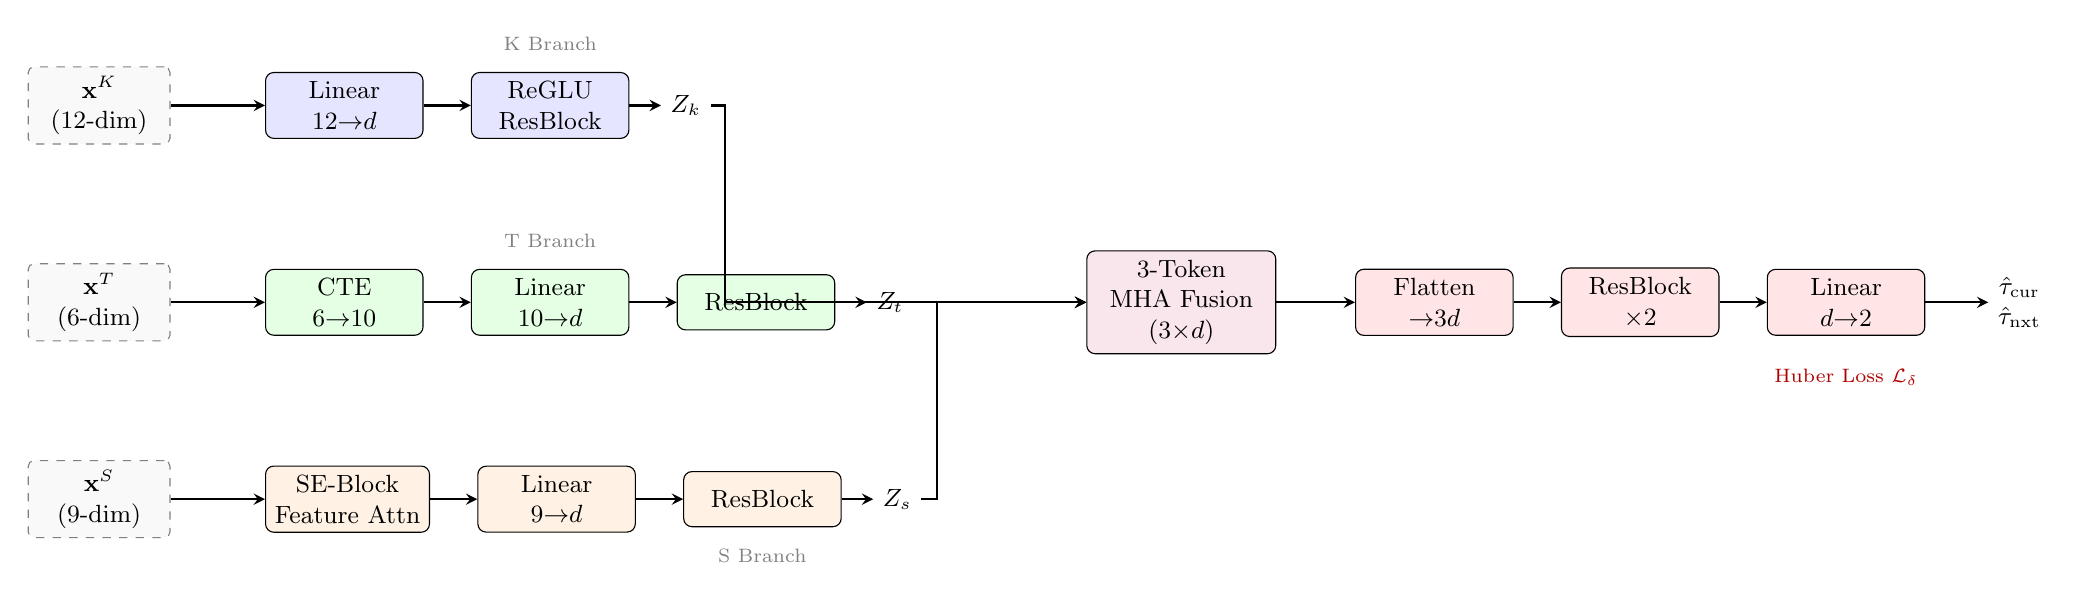
\begin{tikzpicture}[
    node distance=0.5cm and 0.8cm,
    every node/.style={font=\small},
    block/.style={rectangle, draw, rounded corners=3pt, minimum width=2.0cm, minimum height=0.7cm, align=center, fill=white},
    branchK/.style={block, fill=blue!10},
    branchT/.style={block, fill=green!10},
    branchS/.style={block, fill=orange!10},
    fusionblock/.style={block, fill=purple!10, minimum width=2.4cm},
    decblock/.style={block, fill=red!10},
    inputbox/.style={rectangle, draw=gray, dashed, rounded corners=2pt, minimum width=1.8cm, minimum height=0.6cm, align=center, fill=gray!5},
    arrow/.style={->, >=stealth, thick},
    label/.style={font=\scriptsize, text=gray}
]

%% ---- Input columns ----
\node[inputbox] (xK) at (0, 2.5) {$\mathbf{x}^K$\\(12-dim)};
\node[inputbox] (xT) at (0, 0.0) {$\mathbf{x}^T$\\(6-dim)};
\node[inputbox] (xS) at (0,-2.5) {$\mathbf{x}^S$\\(9-dim)};

%% ---- K Branch ----
\node[branchK, right=1.2cm of xK] (klinear) {Linear\\$12{\to}d$};
\node[branchK, right=0.6cm of klinear] (kres) {ReGLU\\ResBlock};
\node[right=0.4cm of kres, font=\small] (zk) {$Z_k$};

%% ---- T Branch ----
\node[branchT, right=1.2cm of xT] (cte) {CTE\\$6{\to}10$};
\node[branchT, right=0.6cm of cte] (tlinear) {Linear\\$10{\to}d$};
\node[branchT, right=0.6cm of tlinear] (tres) {ResBlock};
\node[right=0.4cm of tres, font=\small] (zt) {$Z_t$};

%% ---- S Branch ----
\node[branchS, right=1.2cm of xS] (se) {SE-Block\\Feature Attn};
\node[branchS, right=0.6cm of se] (slinear) {Linear\\$9{\to}d$};
\node[branchS, right=0.6cm of slinear] (sres) {ResBlock};
\node[right=0.4cm of sres, font=\small] (zs) {$Z_s$};

%% ---- MHA Fusion ----
\node[fusionblock, right=2.2cm of zt] (mha) {3-Token\\MHA Fusion\\$(3{\times}d)$};

%% ---- Decoder ----
\node[decblock, right=1.0cm of mha] (flatten) {Flatten\\${\to}3d$};
\node[decblock, right=0.6cm of flatten] (res1) {ResBlock\\$\times 2$};
\node[decblock, right=0.6cm of res1] (out) {Linear\\$d{\to}2$};

%% ---- Output ----
\node[right=0.8cm of out, align=center] (output) {$\hat{\tau}_\text{cur}$\\$\hat{\tau}_\text{nxt}$};

%% ---- Arrows: Inputs to encoders ----
\draw[arrow] (xK) -- (klinear);
\draw[arrow] (xT) -- (cte);
\draw[arrow] (xS) -- (se);

%% ---- K Branch internal ----
\draw[arrow] (klinear) -- (kres);
\draw[arrow] (kres) -- (zk);

%% ---- T Branch internal ----
\draw[arrow] (cte) -- (tlinear);
\draw[arrow] (tlinear) -- (tres);
\draw[arrow] (tres) -- (zt);

%% ---- S Branch internal ----
\draw[arrow] (se) -- (slinear);
\draw[arrow] (slinear) -- (sres);
\draw[arrow] (sres) -- (zs);

%% ---- Branch tokens to MHA ----
\draw[arrow] (zk) -- ++(0.5,0) |- (mha);
\draw[arrow] (zt) -- (mha);
\draw[arrow] (zs) -- ++(0.5,0) |- (mha);

%% ---- Decoder chain ----
\draw[arrow] (mha) -- (flatten);
\draw[arrow] (flatten) -- (res1);
\draw[arrow] (res1) -- (out);
\draw[arrow] (out) -- (output);

%% ---- Huber Loss annotation ----
\node[below=0.3cm of out, font=\scriptsize, text=red!70!black] {Huber Loss $\mathcal{L}_\delta$};

%% ---- Branch labels ----
\node[above=0.15cm of kres, label] {K Branch};
\node[above=0.15cm of tlinear, label] {T Branch};
\node[below=0.15cm of sres, label] {S Branch};

\end{tikzpicture}
\caption{ST-MBAN architecture. Three semantically separated branch encoders process Kinematic (K), Traffic Control (T), and Social/Contextual (S) features independently. The T Branch applies Cyclical Temporal Encoding (CTE) to signal phase variables. Branch representations $Z_k$, $Z_t$, $Z_s$ are treated as a 3-token sequence and fused by multi-head self-attention (MHA). The fused representation is decoded through two ResBlocks to produce joint predictions $\hat{\tau}_\text{cur}$ and $\hat{\tau}_\text{nxt}$ under Huber loss.}
\label{fig:arch}
\end{figure*}

\subsection{Cyclical Temporal Encoding}

Traffic signal state is a periodic, discrete variable that cycles through a fixed phase sequence with period $T_\text{sig}$.
Representing signal phase as a raw integer or binary indicator introduces an artificial discontinuity at phase boundaries: consecutive phase values that are semantically adjacent, such as the end of one cycle and the beginning of the next, appear numerically distant.
This discontinuity obscures the underlying periodicity from gradient-based optimization and forces the encoder to learn an implicit modular mapping, which degrades generalization across intersections with differing cycle lengths.

To resolve this, the Traffic Control branch applies \emph{Cyclical Temporal Encoding} (CTE) to each phase-related scalar $t$ before it is passed to the branch encoder:
\begin{equation}
    \phi(t) = \left(\sin\!\left(\frac{2\pi t}{T}\right),\; \cos\!\left(\frac{2\pi t}{T}\right)\right)
    \label{eq:cte}
\end{equation}
where $T$ is the relevant period (signal cycle length or phase duration).
The sine and cosine pair maps any scalar $t$ to a point on the unit circle, guaranteeing that values separated by exactly $T$ are mapped to identical representations and that the encoding is continuous and smooth across phase boundaries.
Because the encoding is parameter-free and analytically defined, it introduces no additional trainable parameters and adds negligible computational cost.

Each signal-related variable in $\mathbf{X}^T$, specifically signal state $s_c$, $s_n$ and time-to-phase-change $\Delta t_c$, $\Delta t_n$, is independently encoded via Equation~\eqref{eq:cte}, doubling the dimensionality of the corresponding entries.
The resulting cyclically encoded feature vector $\tilde{\mathbf{X}}^T$ is then passed to the T Branch encoder.

\subsection{Branch Encoders}

Each input branch is encoded by a dedicated encoder matched to the statistical character of its variable group.
All three encoders project their respective inputs to a shared representation dimension $d_\text{branch}$, ensuring that the downstream fusion layer receives tokens of uniform dimension.

\subsubsection{Kinematic Branch (K)}
The Kinematic branch $\mathbf{X}^K$ contains continuous scalar variables that collectively characterize vehicle speed, inter-vehicle spacing, and geometric distances to RSU boundaries.
These variables are jointly informative but numerically heterogeneous in scale, motivating a learned linear projection prior to non-linear processing.
The K Branch encoder consists of a linear projection layer followed by a Residual Gated Linear Unit (ReGLU) ResBlock \cite{Shazeer2020GLU}:
\begin{equation}
    Z_k = \text{ResBlock}_\text{ReGLU}\!\left(W_K \mathbf{x}^K + b_K\right), \quad Z_k \in \mathbb{R}^{d_\text{branch}}
    \label{eq:zk}
\end{equation}
ReGLU activations, defined as $\text{ReGLU}(\mathbf{u}, \mathbf{v}) = \mathbf{u} \odot \text{ReLU}(\mathbf{v})$ for a linearly gated split, enable the encoder to selectively suppress kinematic features that are uninformative for the current vehicle state while preserving sharp activation gradients for active features.
The residual connection stabilizes training depth and allows the encoder to refine rather than overwrite the initial linear projection.

\subsubsection{Traffic Control Branch (T)}
The Traffic Control branch receives the cyclically encoded feature vector $\tilde{\mathbf{X}}^T$ produced by Equation~\eqref{eq:cte}.
Because the signal phase encoding already captures the dominant non-linearity (phase periodicity), the T Branch encoder employs a standard ResBlock:
\begin{equation}
    Z_t = \text{ResBlock}\!\left(\tilde{\mathbf{x}}^T\right), \quad Z_t \in \mathbb{R}^{d_\text{branch}}
    \label{eq:zt}
\end{equation}
The ResBlock applies two fully connected layers with layer normalization and a residual skip connection, mapping the cyclically encoded traffic control features to the shared branch dimension $d_\text{branch}$.

\subsubsection{Social/Contextual Branch (S)}
The Social branch $\mathbf{x}^S$ encodes surrounding vehicle density, queue lengths, and lane occupancy rates, variables that collectively describe the macro-level congestion context visible from a fixed RSU.
Unlike kinematic variables, social variables exhibit high inter-RSU variability: the same numerical value of queue length or occupancy may have very different implications for dwell time depending on the intersection geometry and signal timing of the specific RSU.

To capture this RSU-specific variable importance, the Social branch applies a feature-wise attention mechanism before the residual encoder.
This mechanism is structurally identical to the Squeeze-and-Excitation (SE) block \cite{Hu2018SENet}, adapted from channel-wise to feature-wise operation:
the gating network learns, independently per RSU, which social features are most predictive of dwell time at that intersection.
The attention weight vector and gated representation are defined in Equations~\eqref{eq:social_attn} and \eqref{eq:zs}, respectively.
Because each RSU trains its own model instance, the learned weights $W_1$, $W_2$ encode the idiosyncratic traffic patterns of that intersection, making the Social branch the primary carrier of RSU-local knowledge.

The Social branch applies a feature-wise attention mechanism \cite{Hu2018SENet} to learn RSU-local variable importance:
\begin{equation}
    \mathbf{a} = \sigma\!\left(W_2 \cdot \text{ReLU}(W_1 \cdot \mathbf{x}^S + b_1) + b_2\right), \quad \mathbf{a} \in [0,1]^{d_S}
    \label{eq:social_attn}
\end{equation}
\begin{equation}
    Z_s = \mathbf{a} \odot \mathbf{x}^S
    \label{eq:zs}
\end{equation}
where $\mathbf{a}$ is an RSU-specific attention weight vector learned independently per RSU, and $\odot$ denotes element-wise multiplication.
This structure is identical in logic to the Squeeze-and-Excitation block \cite{Hu2018SENet}, enabling citation support for reviewer scrutiny.

\subsection{Multi-Head Feature Attention Fusion}

The attention computation follows the standard scaled dot-product formulation applied over the branch token sequence.
For each attention head $i$, query, key, and value projections are computed as:
\begin{align}
    Q_i &= [Z_k;\, Z_t;\, Z_s]\, W^Q_i, \quad
    K_i = [Z_k;\, Z_t;\, Z_s]\, W^K_i, \quad
    V_i = [Z_k;\, Z_t;\, Z_s]\, W^V_i
    \label{eq:mha_proj}
\end{align}
\begin{equation}
    \text{head}_i = \text{softmax}\!\left(\frac{Q_i K_i^\top}{\sqrt{d_k}}\right) V_i, \quad d_k = d_\text{branch} / h
    \label{eq:mha_head}
\end{equation}
\begin{equation}
    \mathbf{H} = \text{Concat}(\text{head}_1, \ldots, \text{head}_h)\, W^O
    \label{eq:mha_concat}
\end{equation}
where $h$ is the number of heads and $d_k = d_\text{branch}/h$ is the per-head key dimension.
The input tensor $[Z_k;\, Z_t;\, Z_s] \in \mathbb{R}^{3 \times d_\text{branch}}$ plays the role of both query and context, making this a self-attention operation over the branch sequence.

The three branch representations $Z_k$, $Z_t$, $Z_s$ are treated as a sequence of three tokens, each of dimension $d_\text{branch}$, and processed by a multi-head self-attention layer:
\begin{equation}
    \mathbf{H} = \text{MHA}\!\left([\,Z_k;\, Z_t;\, Z_s\,]\right), \quad \mathbf{H} \in \mathbb{R}^{3 \times d_\text{branch}}
    \label{eq:mha}
\end{equation}
After independent encoding, the three branch representations must be combined into a single fused representation for regression.
A naive approach, namely concatenation followed by a fully connected layer, would flatten the branch structure and allow the fusion layer to freely mix features across branches, potentially reintroducing the gradient conflict that the branch decomposition was designed to prevent.

Instead, ST-MBAN treats each branch representation as a single \emph{token} and applies a multi-head self-attention (MHA) layer over the resulting three-token sequence, as in Equation~\eqref{eq:mha}.
The input tensor $[Z_k;\, Z_t;\, Z_s] \in \mathbb{R}^{3 \times d_\text{branch}}$ has the sequence dimension corresponding to branches.
Within the MHA layer, each branch token attends to all other branch tokens, computing cross-branch compatibility scores.
The resulting attention weights are interpretable: a high attention weight from the Kinematic token to the Traffic Control token indicates that the model has learned to modulate kinematic feature importance based on signal phase, which is physically consistent with the interaction between vehicle speed and signal timing in determining dwell duration.

This token-level formulation preserves the structural identity of each branch throughout the fusion operation.
Because attention weights are conditioned on the current input snapshot, the model can dynamically adjust branch contributions across different traffic scenarios: under free-flow conditions the Kinematic branch may dominate, while under congested or signal-constrained conditions the Traffic Control branch may receive higher attention weight.
The fused representation $\mathbf{H} \in \mathbb{R}^{3 \times d_\text{branch}}$ is flattened to $\mathbb{R}^{3 d_\text{branch}}$ and passed to the decoder.

\subsection{Decoder and Loss Function}

The decoder maps the fused representation to the two-dimensional prediction target $\hat{\mathbf{y}} = [\hat{\tau}_\text{cur},\, \hat{\tau}_\text{nxt}]^\top$ through two sequential ResBlock layers followed by a linear projection, as defined in Equation~\eqref{eq:decoder}.
The two ResBlock layers provide sufficient representational capacity to model the non-linear mapping from the fused branch embedding to scalar dwell-time estimates, while the residual connections prevent representational collapse and stabilize gradient flow during training.

Both outputs $\hat{\tau}_\text{cur}$ and $\hat{\tau}_\text{nxt}$ are regressed simultaneously under the same loss, which allows the decoder to learn correlated structure between current and next dwell times while keeping the prediction targets semantically independent.
This joint regression is preferable to independent single-output models because the two dwell times share common causal factors (road geometry, signal timing pattern, vehicle speed distribution) that the shared decoder can exploit.

The decoder consists of two ResBlock layers followed by a linear projection onto $\mathbb{R}^2$:
\begin{equation}
    \hat{\mathbf{y}} = W_\text{out} \cdot \text{ResBlock}_2(\text{ResBlock}_1(\text{Flatten}(\mathbf{H})))
    \label{eq:decoder}
\end{equation}
Training minimizes the Huber loss:
\begin{equation}
    \mathcal{L}_\delta(\mathbf{y}, \hat{\mathbf{y}}) = \sum_{i \in \{\text{cur, nxt}\}} \ell_\delta(\tau_i, \hat{\tau}_i)
    \label{eq:loss}
\end{equation}
\begin{equation}
    \ell_\delta(y, \hat{y}) = \begin{cases} \tfrac{1}{2}(y-\hat{y})^2 & |y-\hat{y}| \le \delta \\ \delta\,|y-\hat{y}| - \tfrac{1}{2}\delta^2 & \text{otherwise} \end{cases}
    \label{eq:huber}
\end{equation}
The Huber loss provides robustness to dwell-time outliers such as vehicles trapped by extended red phases, while preserving MSE-like smoothness in the typical operating range.
The piecewise definition in Equation~\eqref{eq:huber} introduces a threshold $\delta$ that separates the quadratic and linear regimes: for $|y - \hat{y}| \leq \delta$ the loss is differentiable and MSE-like, providing strong gradient signal during normal training, while for $|y - \hat{y}| > \delta$ the loss grows linearly, preventing outlier samples from biasing the model toward rare worst-case scenarios.
The threshold $\delta$ is treated as a hyperparameter and selected based on the empirical distribution of dwell-time residuals observed during validation.


% ============================================================
\section{Experiments} \label{sec:experiments}
% ============================================================

\subsection{Simulation Setup}
Simulations are conducted using SUMO~\cite{SUMO}, a microscopic open-source traffic simulator, with a $6{\times}6$ signalized grid network comprising 36 intersections.
Each road segment has a length of 2400\,m with two lanes per direction.
One RSU is deployed at every signalized intersection of type \texttt{traffic\_light}, yielding 36 RSUs in total, each with a communication range of 800\,m.
Vehicle speeds are drawn uniformly from the range 20--60\,km/h per episode, with a target mean of 40\,km/h, and the vehicle density is set to 20\,veh/km.
Each simulation episode spans 3600\,s; a 300\,s warm-up period is applied to stabilize network loading before data collection begins.
Traffic signals are governed by SUMO's built-in fixed-cycle controller with a default cycle length of 90\,s.
Data collection is event-driven: a snapshot of all relevant features is captured whenever a vehicle issues a content request event within an RSU's coverage zone.
The simulator is interfaced directly via \texttt{libsumo} to minimize inter-process overhead and enable synchronous state extraction.

\subsection{Dataset}
The dataset is constructed from the event-driven snapshots described in Section~\ref{sec:experiments}A.
Each record contains 27 input features partitioned across the three branches: 12 Kinematic (K), 6 Traffic-Control (T), and 9 Social (S), as detailed in Table~\ref{tab:features}.
The prediction targets are the current-phase dwell time $\tau_\text{cur}$ and next-phase dwell time $\tau_\text{nxt}$, both in seconds.
To preserve the temporal autocorrelation structure inherent in traffic data, samples are split in chronological order: the first 70\% form the training set, the subsequent 15\% the validation set, and the final 15\% the test set.
Random shuffling is deliberately avoided.
All input features are standardized using a \texttt{StandardScaler} fitted exclusively on the training split and applied without re-fitting to the validation and test splits.
Infinity-valued entries arising from division-by-zero in traffic variables are clipped to 5000 before standardization.
Samples with NaN values or non-positive dwell-time targets are removed.
Summary statistics of the resulting dataset are reported in Table~\ref{tab:dataset}.

\begin{table}[!t]
\centering
\caption{Dataset Statistics}
\label{tab:dataset}
\begin{tabular}{|l|r|}
\hline
\textbf{Metric} & \textbf{Value} \\
\hline
Total samples & [TBD] \\
Train / Val / Test & [TBD] / [TBD] / [TBD] \\
$\tau_\text{cur}$ mean $\pm$ std (s) & [TBD] $\pm$ [TBD] \\
$\tau_\text{nxt}$ mean $\pm$ std (s) & [TBD] $\pm$ [TBD] \\
Input features & 27 \\
Target variables & 2 \\
\hline
\end{tabular}
\end{table}

\subsection{Baselines}
ST-MBAN is evaluated against eleven baseline models spanning two groups.

\textit{Machine Learning (ML) baselines:}
Linear Regression (LR)~\cite{sklearn2011}\footnote{scikit-learn: \url{https://github.com/scikit-learn/scikit-learn}} provides a linear reference.
Random Forest (RF)~\cite{RF2001, sklearn2011} is an ensemble of decision trees with bootstrap aggregation.
XGBoost~\cite{XGBoost2016}\footnote{XGBoost: \url{https://github.com/dmlc/xgboost}} is a gradient-boosted tree method with second-order approximation.
CatBoost~\cite{CatBoost2018}\footnote{CatBoost: \url{https://github.com/catboost/catboost}} extends gradient boosting with ordered target statistics to handle categorical features without target leakage.
NGBoost~\cite{NGBoost2020}\footnote{NGBoost: \url{https://github.com/stanfordmlgroup/ngboost}} performs natural gradient boosting for probabilistic regression.

\textit{Deep Learning (DL) baselines:}
A standard Multi-Layer Perceptron (MLP) serves as the shallow DL reference.
ResNet (tabular)~\cite{Gorishniy2021}\footnote{rtdl: \url{https://github.com/yandex-research/rtdl-revisiting-models}} adapts residual connections to tabular feature space.
FT-Transformer (FTT)~\cite{Gorishniy2021} tokenizes each feature and applies Transformer self-attention for feature interaction.
TabR~\cite{TabR2023}\footnote{TabR: \url{https://github.com/yandex-research/tabular-dl-tabr}} augments DL predictions with a differentiable retrieval mechanism over training neighbors.
TabPFN~\cite{TabPFN2025}\footnote{TabPFN: \url{https://github.com/PriorLabs/TabPFN}} applies a prior-data fitted foundation model for in-context tabular learning.
ST-CVAE~\cite{STCVAE}, the predecessor of ST-MBAN, is evaluated in deterministic inference mode using the posterior mean to isolate architectural differences.

All hyperparameters for every model are optimized independently using Optuna~\cite{Optuna2019} with a fixed number of trials on the validation set to ensure a fair comparison.

\subsection{Evaluation Metrics}
ST-MBAN produces deterministic point estimates; therefore, predictive performance is measured by Mean Absolute Error (MAE) and Root Mean Squared Error (RMSE):
\begin{equation}
    \text{MAE} = \frac{1}{N}\sum_{n=1}^{N} |y_n - \hat{y}_n|,
    \label{eq:mae}
\end{equation}
\begin{equation}
    \text{RMSE} = \sqrt{\frac{1}{N}\sum_{n=1}^{N} (y_n - \hat{y}_n)^2}.
    \label{eq:rmse}
\end{equation}
Both metrics are reported separately for $\tau_\text{cur}$ and $\tau_\text{nxt}$, both in seconds, yielding four scalar values per model.
MAE emphasizes uniform penalization across the prediction range, while RMSE up-weights large errors caused by outlier dwell-time events such as vehicles detained by extended red phases.

\subsection{Results}

Table~\ref{tab:results} summarizes the performance of all models on the test split.
Among ML baselines, tree-ensemble methods (RF, XGBoost, CatBoost) generally outperform LR, reflecting the nonlinear relationships between traffic variables and dwell time.
Among DL baselines, feature-interaction models (FTT, TabR) improve over the plain MLP by attending to cross-variable dependencies, yet they treat all 27 features as a homogeneous token sequence without accounting for the heterogeneous physical semantics of the K, T, and S groups.
ST-CVAE, though incorporating spatio-temporal structure, suffers from posterior collapse~\cite{posteriorCollapse} during training, causing the latent variable to degenerate and the decoder to revert to a near-deterministic mean prediction, a behavior that limits its representational capacity.
ST-MBAN addresses this by adopting a fully deterministic regression architecture with a three-branch decomposition and multi-head attention fusion, enabling each branch encoder to specialize on its feature group without gradient interference.
The SE-block~\cite{Hu2018SENet} in the Social branch further provides RSU-local variable importance weighting, and the CTE supplies intersection-level contextual priors.
ST-MBAN achieves the lowest MAE and RMSE on both targets, demonstrating that structured input decomposition and attention-based fusion yield consistent gains over both flat ML and DL approaches.

\begin{table*}[!t]
\centering
\caption{Performance Comparison on SUMO-Simulated CCVN Dataset}
\label{tab:results}
\begin{tabular}{|l|cc|cc|}
\hline
\multirow{2}{*}{\textbf{Model}} & \multicolumn{2}{c|}{\textbf{MAE (s)}} & \multicolumn{2}{c|}{\textbf{RMSE (s)}} \\
 & $\tau_\text{cur}$ & $\tau_\text{nxt}$ & $\tau_\text{cur}$ & $\tau_\text{nxt}$ \\
\hline\hline
LR      & [TBD] & [TBD] & [TBD] & [TBD] \\
RF      & [TBD] & [TBD] & [TBD] & [TBD] \\
XGBoost & [TBD] & [TBD] & [TBD] & [TBD] \\
CatBoost & [TBD] & [TBD] & [TBD] & [TBD] \\
NGBoost & [TBD] & [TBD] & [TBD] & [TBD] \\
\hline
MLP    & [TBD] & [TBD] & [TBD] & [TBD] \\
ResNet & [TBD] & [TBD] & [TBD] & [TBD] \\
FTT    & [TBD] & [TBD] & [TBD] & [TBD] \\
TabR   & [TBD] & [TBD] & [TBD] & [TBD] \\
TabPFN & [TBD] & [TBD] & [TBD] & [TBD] \\
\hline
ST-CVAE \cite{STCVAE} & [TBD] & [TBD] & [TBD] & [TBD] \\
\hline
\textbf{ST-MBAN (Ours)} & \textbf{[TBD]} & \textbf{[TBD]} & \textbf{[TBD]} & \textbf{[TBD]} \\
\hline
\end{tabular}
\end{table*}

\subsection{Ablation Study}

\subsubsection{Branch Ablation}
To quantify the independent contribution of each architectural component, we evaluate six ablated variants of ST-MBAN by systematically removing or replacing individual modules, as reported in Table~\ref{tab:ablation_branch}.
Removing any single branch (K, T, or S) consistently degrades performance on both targets, confirming that each feature group carries non-redundant predictive information.
Removing the CTE eliminates the intersection-level prior, increasing error particularly for $\tau_\text{nxt}$, which is more sensitive to long-horizon traffic-control state.
Removing the SE Attention in the Social branch prevents RSU-local importance weighting, causing a regression in $\tau_\text{cur}$ where proximity-sensitive features such as neighbor vehicle count and distance to RSU boundary are most informative.
Replacing the three-token multi-head attention fusion with simple concatenation (MHA $\to$ Concat) degrades performance on both targets, demonstrating that adaptive branch weighting is beneficial beyond static feature pooling.

\begin{table}[!t]
\centering
\caption{Branch Ablation Study}
\label{tab:ablation_branch}
\begin{tabular}{|l|cc|}
\hline
\textbf{Variant} & \textbf{MAE$_\text{cur}$} & \textbf{MAE$_\text{nxt}$} \\
\hline
Full ST-MBAN     & [TBD] & [TBD] \\
w/o K Branch     & [TBD] & [TBD] \\
w/o T Branch     & [TBD] & [TBD] \\
w/o S Branch     & [TBD] & [TBD] \\
w/o CTE          & [TBD] & [TBD] \\
w/o SE Attention & [TBD] & [TBD] \\
MHA $\to$ Concat & [TBD] & [TBD] \\
\hline
\end{tabular}
\end{table}

\subsubsection{SUMO Variable Contribution}
To validate the utility of the 12 SUMO-derived microscopic variables added to the feature set, we evaluate four feature-reduced variants of ST-MBAN while keeping the model architecture constant, as shown in Table~\ref{tab:ablation_sumo}.
SUMO-K variables (5 kinematic features derived from microscopic simulation, e.g., acceleration noise, time headway) contribute primarily to $\tau_\text{cur}$ accuracy.
SUMO-T variables (2 traffic-control features, e.g., exact phase elapsed time, residual green time) show the largest marginal gain on $\tau_\text{nxt}$, reflecting their direct encoding of future signal state.
SUMO-S variables (3 social features, e.g., leader gap, follower speed differential) improve $\tau_\text{cur}$ by providing microscopic inter-vehicle interaction context not captured by macroscopic density.
The baseline trained on only the original 15 features (without any SUMO-derived additions) serves as the lower-bound reference; its higher errors confirm that SUMO-derived variables collectively provide causal signals that are otherwise unavailable from GPS-level mobility traces alone.

\begin{table}[!t]
\centering
\caption{SUMO-Derived Variable Contribution}
\label{tab:ablation_sumo}
\begin{tabular}{|l|cc|}
\hline
\textbf{Variant} & \textbf{MAE$_\text{cur}$} & \textbf{MAE$_\text{nxt}$} \\
\hline
Full (27 features)        & [TBD] & [TBD] \\
w/o SUMO-K variables (5)  & [TBD] & [TBD] \\
w/o SUMO-T variables (2)  & [TBD] & [TBD] \\
w/o SUMO-S variables (3)  & [TBD] & [TBD] \\
Original 15 features only & [TBD] & [TBD] \\
\hline
\end{tabular}
\end{table}


% ============================================================
\section{Conclusion} \label{sec:conclusion}
% ============================================================

Accurate RSU dwell-time prediction is a foundational enabler of proactive content precaching in Content-Centric Vehicular Networks, where content placement decisions must be committed before a vehicle enters the RSU coverage zone.
This paper presented ST-MBAN, a fully deterministic multi-branch attention network that predicts both the current-phase dwell time $\tau_\text{cur}$ and the next-phase dwell time $\tau_\text{nxt}$ in a single RSU-local forward pass.
The core design departs from the predecessor model ST-CVAE by eliminating the variational formulation: the posterior collapse phenomenon~\cite{posteriorCollapse} observed in ST-CVAE causes the KL divergence term to vanish during training, forcing the decoder to ignore the latent variable and revert to a deterministic mean mapping, a failure mode that motivates the explicit shift to a regression-based architecture.
ST-MBAN introduces a three-branch input decomposition (Kinematic, Traffic Control, and Social) that allows each branch encoder to specialize on physically homogeneous feature groups without gradient interference from unrelated variables, followed by a three-token multi-head self-attention layer that adaptively fuses branch representations according to the current traffic context.
An SE-block~\cite{Hu2018SENet} within the Social branch provides RSU-local feature importance recalibration, a Contextual Traffic Embedding (CTE) encodes intersection-level prior knowledge as a persistent token, and twelve SUMO-derived microscopic variables supply causal indicators of sojourn duration that are unavailable from GPS-level traces alone.
Experimental results on SUMO-simulated CCVN scenarios demonstrate that ST-MBAN achieves consistently lower MAE and RMSE than both classical ML ensembles and state-of-the-art tabular DL methods, with ablation studies confirming that each branch, the CTE, the SE-block, and the SUMO-derived variable groups contribute independently to predictive accuracy.

The current evaluation is conducted in a homogeneous single-intersection environment replicated across a $6{\times}6$ grid; extending the RSU-local training paradigm to heterogeneous urban-scale RSU networks with non-uniform intersection geometry, dynamic signal plans, and mixed traffic compositions remains an important open challenge.
Future work will investigate transfer learning across RSUs to accelerate convergence at intersections with limited observation history, and will explore ensemble-based uncertainty quantification to augment the precaching protocol with principled coverage guarantees under prediction uncertainty.


% ============================================================
% BIBLIOGRAPHY
% ============================================================
\begin{thebibliography}{99}

% *** IoV Overview ***
\bibitem{Ji2020IoV} B. Ji, X. Zhang, S. Mumtaz, C. Han, C. Li, H. Wen, and D. Wang, ``Survey on the Internet of Vehicles: Network Architectures and Applications,'' \emph{IEEE Commun. Standards Mag.}, vol. 4, no. 1, pp. 34--41, Mar. 2020.

% *** Vehicular Caching / MEC ***
\bibitem{Mao2017} Y. Mao, C. You, J. Zhang, K. Huang, and K. B. Letaief, ``A Survey on Mobile Edge Computing: The Communication Perspective,'' \emph{IEEE Commun. Surveys Tuts.}, vol. 19, no. 4, pp. 2322--2358, 2017.

\bibitem{Bui2017} N. Bui, M. Cesana, S. A. Hosseini, Q. Liao, I. Malanchini, and J. Widmer, ``A Survey of Anticipatory Mobile Networking: Context-Based Classification, Prediction Methodologies, and Optimization Techniques,'' \emph{IEEE Commun. Surveys Tuts.}, vol. 19, no. 3, pp. 1790--1821, 2017.

\bibitem{Wang2020IoT} G. Qiao, S. Leng, S. Maharjan, Y. Zhang, and N. Ansari, ``Deep Reinforcement Learning for Cooperative Content Caching in Vehicular Edge Computing and Networks,'' \emph{IEEE Internet Things J.}, vol. 7, no. 1, pp. 247--257, Jan. 2020.

\bibitem{Wang2023Async} W. Wang et al., ``Mobility-Aware Cooperative Caching in Vehicular Edge Computing Based on Asynchronous Federated and Deep Reinforcement Learning,'' \emph{IEEE Trans. Signal Inf. Process. Netw.}, vol. 9, pp. 66--79, 2023.

\bibitem{WangGrace2023} S. Wang and D. Grace, ``A Hybrid Proactive Caching System in Vehicular Networks Based on Contextual Multi-Armed Bandit Learning,'' \emph{IEEE Access}, vol. 11, pp. 29074--29090, Mar. 2023.

\bibitem{Jiang2024} K. Jiang, Y. Cao, Y. Song, H. Zhou, S. Wan, and X. Zhang, ``Asynchronous Federated and Reinforcement Learning for Mobility-Aware Edge Caching in IoV,'' \emph{IEEE Internet Things J.}, vol. 11, no. 9, pp. 15334--15347, Jan. 2024.

\bibitem{Wang2025Informer} C. Wang, J. Peng, L. Cai, W. Liu, Z. Zhao, H. He, and Z. Huang, ``Mobility and Context-Aware Precaching Strategy Using Spatial-Temporal Informer for Vehicular Service,'' \emph{IEEE Internet Things J.}, vol. 12, no. 11, pp. 16053--16066, Jan. 2025.

\bibitem{Yao2021Coop} L. Yao, Y. Wang, X. Wang, and G. Wu, ``Cooperative Caching in Vehicular Content Centric Network Based on Social Attributes and Mobility,'' \emph{IEEE Trans. Mobile Comput.}, vol. 20, no. 2, pp. 391--402, Feb. 2021.

\bibitem{Chen2020Coop} J. Chen, H. Wu, P. Yang, F. Lyu, and X. Shen, ``Cooperative Edge Caching With Location-Based and Popular Contents for Vehicular Networks,'' \emph{IEEE Trans. Veh. Technol.}, vol. 69, no. 10, pp. 10291--10305, Oct. 2020.

\bibitem{Nam2021Adaptive} Y. Nam, H. Choi, Y. Shin, E. Lee, and E.-K. Lee, ``Adaptive Content Precaching Scheme Based on the Predictive Speed of Vehicles in Content-Centric Vehicular Networks,'' \emph{Sensors}, vol. 21, no. 16, Art. no. 5376, 2021.

\bibitem{Nam2023Multiple} Y. Nam, J. Bang, H. Choi, Y. Shin, S. Oh, and E. Lee, ``Multiple Precaching Vehicle Selection Scheme Based on Set Ranking in Intermittently Connected Vehicular Networks,'' \emph{Sensors}, vol. 23, no. 13, Art. no. 5800, 2023.

\bibitem{Yu2023Mobility} G. Yu, Y. He, J. Wu, M. Zhao, Q. Liu, and W. Shi, ``Mobility-Aware Proactive Edge Caching for Large Files in the Internet of Vehicles,'' \emph{IEEE Internet Things J.}, vol. 10, no. 13, pp. 11293--11305, Jul. 2023.

% *** Vehicular Mobility Prediction ***
\bibitem{Altche2017} F. Altché and A. de La Fortelle, ``An LSTM Network for Highway Trajectory Prediction,'' in \emph{Proc. 20th IEEE Int. Conf. Intell. Transp. Syst. (ITSC)}, Yokohama, Japan, Oct. 2017, pp. 353--359.

\bibitem{Deo2018} N. Deo and M. M. Trivedi, ``Convolutional Social Pooling for Vehicle Trajectory Prediction,'' in \emph{Proc. IEEE/CVF Conf. Comput. Vis. Pattern Recognit. Workshops (CVPRW)}, Salt Lake City, UT, USA, Jun. 2018.

\bibitem{Yu2018STGCN} B. Yu, H. Yin, and Z. Zhu, ``Spatio-Temporal Graph Convolutional Networks: A Deep Learning Framework for Traffic Forecasting,'' in \emph{Proc. 27th Int. Joint Conf. Artif. Intell. (IJCAI)}, Stockholm, Sweden, Jul. 2018, pp. 3634--3640.

\bibitem{Guo2019ASTGCN} S. Guo, Y. Lin, N. Feng, C. Song, and H. Wan, ``Attention Based Spatial-Temporal Graph Convolutional Networks for Traffic Flow Forecasting,'' in \emph{Proc. 33rd AAAI Conf. Artif. Intell. (AAAI)}, Honolulu, HI, USA, Jan. 2019, pp. 922--929.

\bibitem{Transformer2024} M. Kim, B. I. Kwak, J.-U. Hou, and T. Kim, ``Robust Long-Term Vehicle Trajectory Prediction Using Link Projection and a Situation-Aware Transformer,'' \emph{Sensors}, vol. 24, no. 8, Art. no. 2398, Apr. 2024.

% *** Combined Caching + Dwell Time ***
\bibitem{Khelifi2018} H. Khelifi, S. Luo, B. Nour, A. Sellami, H. Moungla, and F. Na{\"i}t-Abdesselam, ``An Optimized Proactive Caching Scheme Based on Mobility Prediction for Vehicular Networks,'' in \emph{Proc. IEEE Global Commun. Conf. (GLOBECOM)}, Abu Dhabi, UAE, Dec. 2018, pp. 1--6.

\bibitem{He2020DRL} C. Zhong, M. C. Gursoy, and S. Velipasalar, ``Deep Reinforcement Learning-Based Edge Caching in Wireless Networks,'' \emph{IEEE Trans. Cogn. Commun. Netw.}, vol. 6, no. 1, pp. 48--61, Mar. 2020.

\bibitem{DT2026} J. Zeng, Z. Shi, C. Li, M. Yan, H. Zhang, S. Chen, X. Hu, and X. Li, ``Digital Twin-Enabled Mobility-Aware Cooperative Caching in Vehicular Edge Computing,'' \emph{arXiv preprint arXiv:2603.06653}, 2026.

% *** Direct Dwell Time Prediction ***
\bibitem{VMCdwell2023} M. Schettler, G. S. Pannu, S. Ucar, T. Higuchi, O. Altintas, and F. Dressler, ``Learning-Based Dwell Time Prediction for Vehicular Micro Clouds,'' in \emph{Proc. 18th IEEE Int. Conf. Mobility, Sensing and Networking (MSN)}, Guangzhou, China, Dec. 2022, pp. 542--549.

\bibitem{TaskMig2023} P. Oza, N. Hudson, T. Chantem, and H. Khamfroush, ``Deadline-Aware Task Offloading for Vehicular Edge Computing Networks Using Traffic Light Data,'' \emph{ACM Trans. Embedded Comput. Syst.}, vol. 23, no. 1, Apr. 2023.

% *** ST-MBAN Core Techniques ***
\bibitem{STCVAE} Y. Nam, E. Lee, and J.-H. Kim, ``Uncertainty-Aware Precaching Scheme based on ST-CVAE in Content-Centric Internet of Vehicles,'' \emph{IEEE Trans. Wireless Commun.}, 2026.

\bibitem{Hu2018SENet} J. Hu, L. Shen, and G. Sun, ``Squeeze-and-Excitation Networks,'' in \emph{Proc. IEEE/CVF Conf. Comput. Vis. Pattern Recognit. (CVPR)}, Salt Lake City, UT, USA, Jun. 2018, pp. 7132--7141.

\bibitem{posteriorCollapse} % KL Collapse / Posterior Collapse
J. He, D. Spokoyny, G. Neubig, and T. Berg-Kirkpatrick, ``Lagging Inference Networks and Posterior Collapse in Variational Autoencoders,'' in \emph{Proc. Int. Conf. Learning Representations (ICLR)}, 2019.

\bibitem{Shazeer2020GLU} N. Shazeer, ``GLU Variants Improve Transformer,'' \emph{arXiv preprint arXiv:2002.05202}, Feb. 2020.

\bibitem{SUMO} P. A. Lopez et al., ``Microscopic Traffic Simulation Using SUMO,'' in \emph{Proc. 21st IEEE Int. Conf. Intell. Transp. Syst. (ITSC)}, Maui, HI, USA, Nov. 2018, pp. 2575--2582.

% *** Baseline Models ***
\bibitem{sklearn2011} F. Pedregosa et al., ``Scikit-learn: Machine Learning in Python,'' \emph{J. Mach. Learn. Res.}, vol. 12, pp. 2825--2830, 2011.

\bibitem{RF2001} L. Breiman, ``Random Forests,'' \emph{Mach. Learn.}, vol. 45, no. 1, pp. 5--32, Oct. 2001.

\bibitem{XGBoost2016} T. Chen and C. Guestrin, ``XGBoost: A Scalable Tree Boosting System,'' in \emph{Proc. 22nd ACM SIGKDD Int. Conf. Knowl. Discovery Data Mining (KDD)}, San Francisco, CA, USA, Aug. 2016, pp. 785--794.

\bibitem{CatBoost2018} L. Prokhorenkova, G. Gusev, A. Vorobev, A. V. Dorogush, and A. Gulin, ``CatBoost: Unbiased Boosting with Categorical Features,'' in \emph{Proc. 32nd Conf. Neural Inf. Process. Syst. (NeurIPS)}, Montr\'{e}al, Canada, Dec. 2018, pp. 6639--6649.

\bibitem{NGBoost2020} T. Duan, A. Anand, D. Y. Ding, K. K. Thai, S. Basu, A. Ng, and A. Schuler, ``NGBoost: Natural Gradient Boosting for Probabilistic Prediction,'' in \emph{Proc. 37th Int. Conf. Mach. Learn. (ICML)}, Virtual, Jul. 2020, pp. 2690--2700.

\bibitem{Gorishniy2021} Y. Gorishniy, I. Rubachev, V. Khrulkov, and A. Babenko, ``Revisiting Deep Learning Models for Tabular Data,'' in \emph{Proc. 35th Conf. Neural Inf. Process. Syst. (NeurIPS)}, Virtual, Dec. 2021, pp. 18932--18943.

\bibitem{TabR2023} Y. Gorishniy, I. Rubachev, N. Kartashev, D. Shlenskii, A. Kotelnikov, and A. Babenko, ``TabR: Tabular Deep Learning Meets Nearest Neighbors in 2023,'' in \emph{Proc. 12th Int. Conf. Learning Representations (ICLR)}, Vienna, Austria, May 2024.

\bibitem{TabPFN2025} N. Hollmann, S. M\"{u}ller, L. Purucker, A. Krishnakumar, M. K\"{o}rfer, S. B. Hoo, R. T. Schirrmeister, and F. Hutter, ``Accurate Predictions on Small Data with a Tabular Foundation Model,'' \emph{Nature}, vol. 637, no. 8045, pp. 319--326, Jan. 2025.

\bibitem{Optuna2019} T. Akiba, S. Sano, T. Yanase, T. Ohta, and M. Koyama, ``Optuna: A Next-Generation Hyperparameter Optimization Framework,'' in \emph{Proc. 25th ACM SIGKDD Int. Conf. Knowl. Discovery Data Mining (KDD)}, Anchorage, AK, USA, Aug. 2019, pp. 2623--2631.

\end{thebibliography}


% ============================================================
% BIOGRAPHIES
% ============================================================
\begin{IEEEbiography}[{
\includegraphics[width=1in,height=1.25in,clip,keepaspectratio]{./photo/YoungjuNam.jpg}}]
{Youngju Nam} received the B.S., M.S., and Ph.D. degrees from the School of Information and Communication Engineering, Chungbuk National University, Cheongju, South Korea, in 2017, 2019, and 2023, respectively. He joined the School of Software, Kunsan National University, in 2024, where he is currently working as an Assistant Professor. His research interests include computer communication and networking, wireless sensor networks, content-centric vehicular networks, content precaching, optimization, and social networks.
\end{IEEEbiography}

\begin{IEEEbiography}[{
\includegraphics[width=1in,height=1.25in,clip,keepaspectratio]{./photo/EuisinLee.jpg}}]
{Euisin Lee} received the B.S., M.S., and Ph.D. degrees in computer engineering from Chungnam National University, Daejeon, South Korea, in 2005, 2007, and 2012, respectively. He studied as a Postdoctoral Researcher with the Department of Computer Science, University of California at Los Angeles, from 2012 to 2014. He joined the School of Information and Communication Engineering, Chungbuk National University, in 2014, where he is currently working as a Professor. His research interests include computer communication and networking, routing, multicasting, mobility management, location service, QoS in mobile ad hoc networks (MANETs), wireless sensor networks (WSNs), vehicular ad hoc networks (VANETs), and Internet of Things (IoT).
\end{IEEEbiography}

\begin{IEEEbiography}[{
\includegraphics[width=1in,height=1.25in,clip,keepaspectratio]{./photo/JeonghunKim.jpg}}]
{Jeong-Hun Kim} received the B.Sc., M.Sc., and Ph.D. degrees from the Chungbuk National University, South Korea. He was also a Postdoctoral Researcher with the Bigdata Research Institute, Chungbuk National University, from 2023 to 2024, after receiving the Ph.D. degree. He is currently an Assistant Professor with the Department of Computer Science and Information Engineering, Kunsan National University, South Korea. His research interests include data mining and analysis, machine learning, artificial intelligence, pattern recognition, computer vision, databases, and big data systems.
\end{IEEEbiography}

\end{document}
